\documentclass[11pt]{article}
\usepackage{enumitem}
%\setlist[itemize]{nosep}       % no extra separation
%\setlist[enumerate]{nosep}
%\setlist[itemize]{topsep=0pt}	% no top separation
%\setlist[enumerate]{topsep=0pt}

\usepackage[margin=1in]{geometry}
\usepackage{tikz}
\usepackage{mathtools}
\usepackage[final]{pdfpages}
\date{}

\begin{document}

\begin{center}
\noindent{\bf {\LARGE COMP 3804/Math 3804: Assignment 1}}\\
\vspace{0.5cm}
{\bf Due Date: Sunday, October $2^{nd}$ at 11:59PM}
\end{center}
\noindent School of Computer Science\hfill{Carleton University}

\noindent \hrulefill

Your assignment should be submitted online on Brightspace as a single .pdf file.  The filename should contain your name and student number. No late assignments will be accepted.You can type your assignment or you can upload a scanned copy of it.  Please, use a good image capturing device. Make sure that your upload is clearly readable. If it is difficult to read, it will not be graded.

%%%%%%%%%%%% NEW SECTION %%%%%%%%%%%%%%%%%
\section*{Question 1 [15 marks]}
Consider the following (not so great) algorithm defined on  a set S of $n$ numbers; assume that $n = 3k +1$, for some non-negative integer $k$. 

For i = 1 to $\lfloor (n/3) \rfloor$  do

	\indent  \indent  STEP 1:  in linear time (in the size of S), find and then delete  both min- and max-element 	\indent  \indent\indent from S
	
 	\indent  \indent STEP 2: Again, in linear time, find and then delete from S  (as updated by STEP 1) \indent  \indent\indent   (just) the max-element.
 
\begin{enumerate}[label=\Roman*.]
	\item 

 	\noindent First, what does  this algorithm do more precisely? (It might help you, to first think about what the algorithm does if you were to  omit Step 2. Do {\bf not} write this as part of your solution.)
		\item 
\noindent Then, write this algorithm in more detailed pseudo-code (filling in the min and max finding, in particular). Also make sure that you take care of the boundary/terminating conditions. 
	\item 
	What is the time complexity of this (bad) algorithm?
	\item 
\noindent   Then, prove  that  this algorithm correctly finds that element  of a set of $n$ elements as determined by you in Part I.
\end{enumerate} 	




%%%%%%%%%%%% NEW SECTION %%%%%%%%%%%%%%%%%
\section*{Question 2 [11 marks]}
Implement the two algorithms presented in class for computing Finonacci numbers, fib1 and fib2 and the direct way using the Golden Ratio.

Each time you compute a Fibonacci number, measure how many milliseconds it takes, and print this timing information. There is a Java function, System.currentTimeMillis(), which returns a long result; call it once before you do the computation, and a second time after you do the computation; subtract to get the elapsed time. Be careful to measure only the computation time; any changes to the GUI should be made either before or after you start measuring. Do not do anything else on your computer. 
From time to time, your computer will do garbage collection, this may explain strange timing results.

What is the maximum value of $n$ for which you can compute Fibonacci? How long does it take for each $n$ that you can compute?
Hand in a listign of your code and the timing results.

%
\section*{Question 3 [34 marks]}
(See also the Tutorial on recurrences)

For the following we will assume that T(1) =1. (If required, you can also assume that T($k$) = O(1), for any constant $k$.) 
For 1-3, "solve" means provide a big-oh bound. 

  \begin{enumerate}
  	\item
  	Solve, by unfolding also known as the iterative method (or repeatedly applyong the recurrence relation):
  \begin{itemize}
  	\item[a.]     $T(n)=T(n-2)+n$.
  	\item[b.] $T(n)=2T(n/4)+n$.
\end{itemize}
   	\item
Now, solve by applying  the recursion tree method:
\begin{itemize}
	\item[a.]     $T(n)=T(n-2)+n$.
		\item[b.] $T(n)=4T(n/4)+n$.
	\item[c.] $T(n)=2T(n/4)+n$.
 
\end{itemize}
   	\item
   	Next, solve by guessing the solution and then proving it using induction:
   	\begin{itemize}
   		\item[a.]     $T(n)=8T(n/8)+n$.
   	   		\item[b.]     $T(n)=T(n/2)+log \ n$.
   	   		  \item[c.]     $T(n)=T(n/2^n) +1$.
   	\end{itemize}
   
  	\item
\noindent  Finally, apply the Master Theorem (in its general form), where possible, to solve the following recurrence relations and give a $\Theta$-bound for each of them. If the master's theorem is not applicable, state why and then solve the recurrence using another method that we learned in class. 
\begin{itemize}
    \item[a.] $T(n)=T(n-4)+n$.
    \item[b.] $T(n)=T(9n/3)+n^2$.
    \item[c.]  $T(n)=T(16n/4)+n^2$.
    \item[d.] $T(n)=7T(n/3)+n^2$.
     \item[e.]$T(n)=2^nT(n/2)+O(1)$
     \item[f.] $T(n)=cT(n/c)+ n$   for some positive integer c.
     \item[g.] $T(n)=2T(n/4)+n^{0.6}$.

   
\end{itemize}
\item
\begin{itemize}
\item[a.]What can you say about the time complexity of an algorithm whose running time is given by this recurrence $T(n)=2T(n)+O(\log^2 n)$?

    \item[b.] Which method might be most appropriate to solve the following recurrence? Use it to give its solution. $T(n)=T(n/4)+T(3n/4)+ n$


\end{itemize}
\end{enumerate}

%%%%%%%%%%%% NEW SECTION %%%%%%%%%%%%%%%%%
\section*{Question 4 [15 marks]}
DT claims that he has a data structure that he can create in O(n) time and on which he can perform the operation DeleteMin using $o(log n)$ comparisons. (note the little-oh)

(a) What could you say about the number of comparisons  used by the most efficient sorting algorithm designed based on DT's claim?  Argue.

(b) Based (a) argue that DT must be lying.

%%%%%%%%%%%% NEW SECTION %%%%%%%%%%%%%%%%%
\section*{Question 5 [25 marks]}
Informally, a convex polygon is a (non self-intersecting) polygon in which each interior angle is less than $180^o$.  
\begin{itemize}
	\item
	Draw a convex polygon  based on that definition.
	\item
	Draw a self-interecting polygon.
\end{itemize}

The convex hull of a set of points $S$  is the smallest convex polygon containing all points of $S$ (no point of $S$ is outside the convex hull; the vertices of the polygon are poinst from $S$). (Without handing this in, draw examples for yourself.)

\begin{itemize}
	
	\item A property of the convex hull  is that, for each edge $e$ of  the convex hull polygon, all points of $S$ are on one side of the (infinite) line drawn through $e$ (some points may be on the line). Draw  this  and hand in with your solution.
	
	 \noindent  Now, design a simple algorithm that uses this property. Prove its correctness and establish its time complexity. 
	  \item Let us see if we can do better. You are given two linear-time algorithms which you can just use without having to give pseudocode nor prove their correctness.  (Like use as a black box)
	  
	  	\noindent\noindent The first one is  a median finding algorithm. The median of a set of $n$ numbers  is the element for which $\lfloor(n/2) \rfloor $ are less than or equal to it and the remaing elements are larger than it.
	  	
	  		\begin{figure}
	  		\centerline{\resizebox{!}{0.7\textwidth}{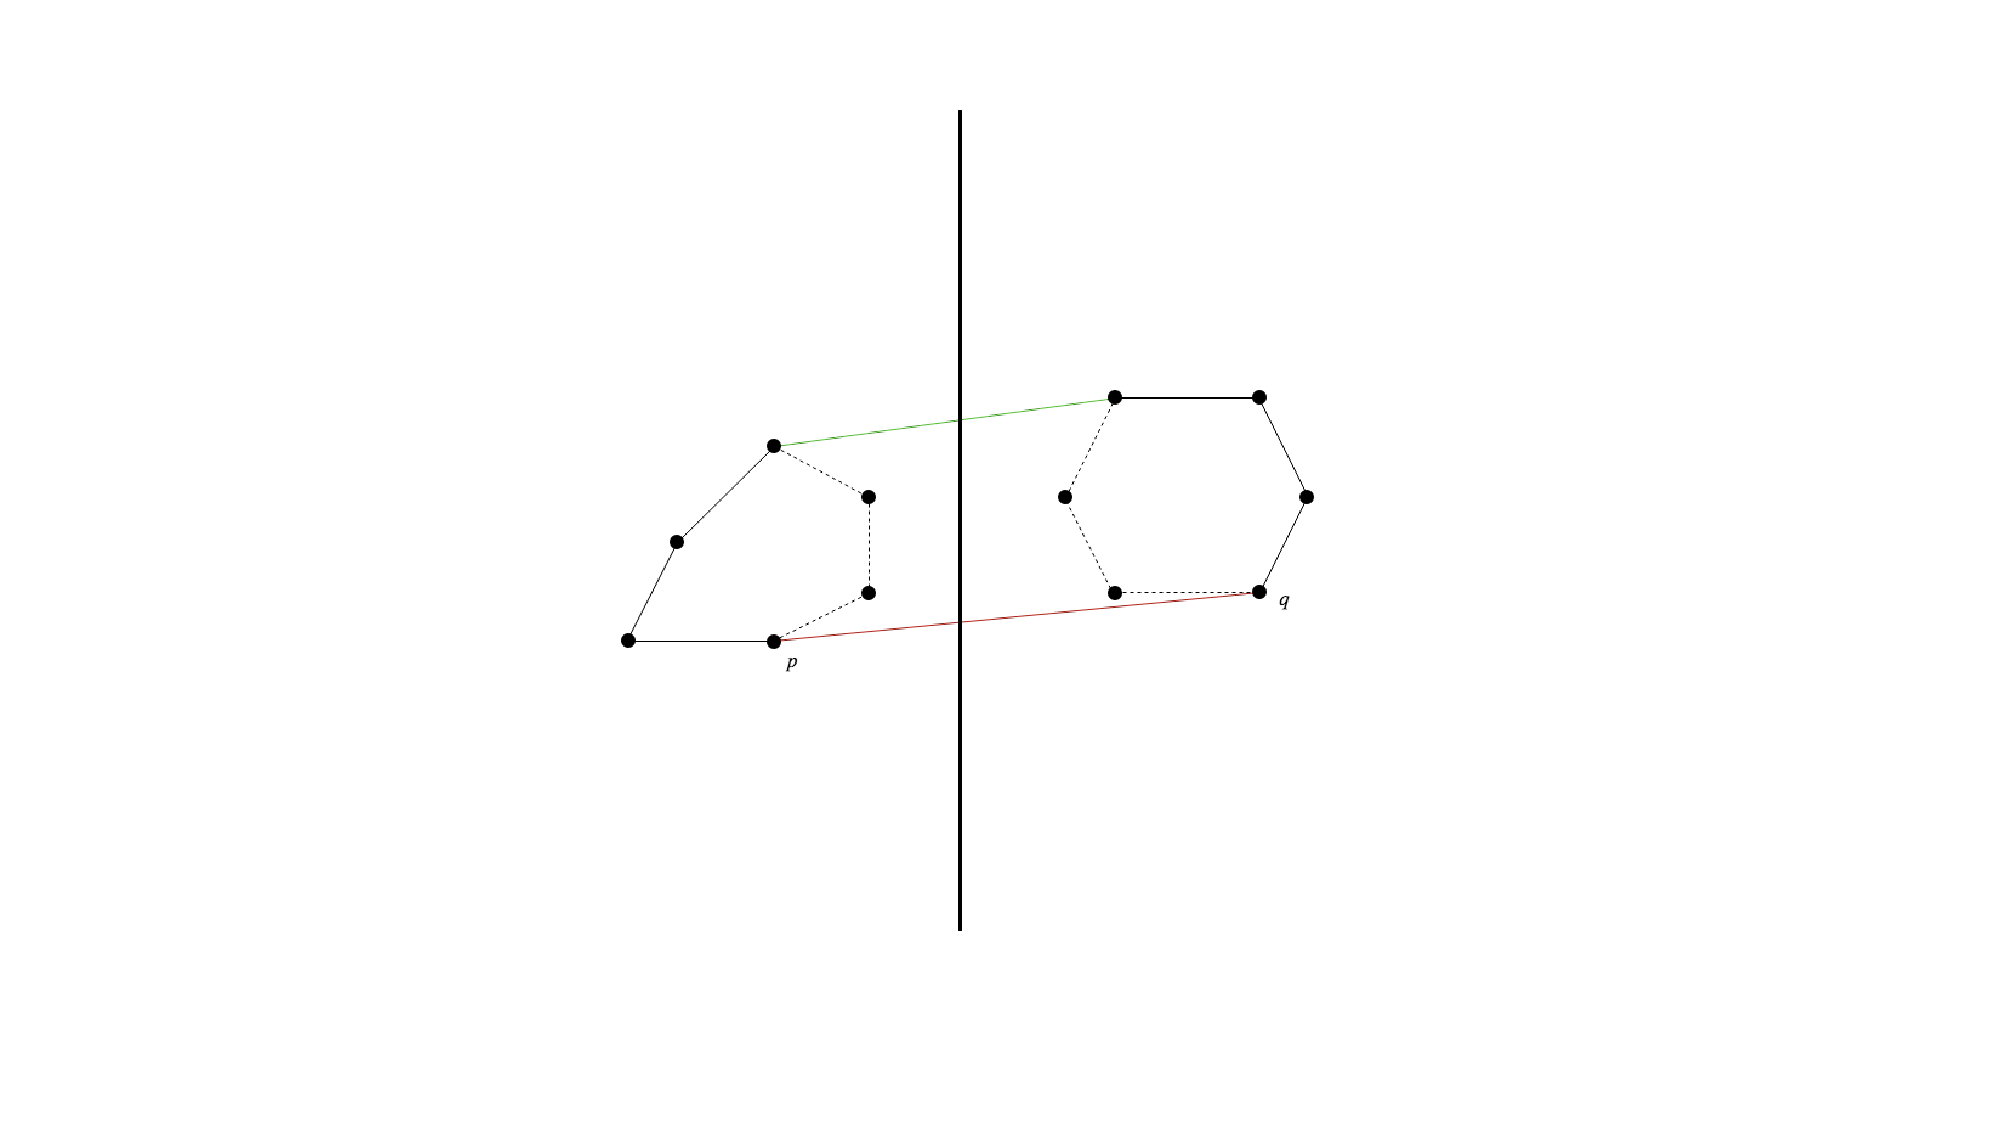
\includegraphics{convexpolygon-merging.pdf}}}
	  		\caption{For Question 5: Merging two Convex Hulls separted by a vertical line}
	  		\label{fig:convexpolygon-merging}
	  	\end{figure}
	  	
	  		\noindent\noindent  The second one computes the convex hull of two point sets for which we are given their convex hulls. The points sets here are assumend to be separated by a vertical line.  See Figure \ref{fig:convexpolygon-merging}.
	  	%	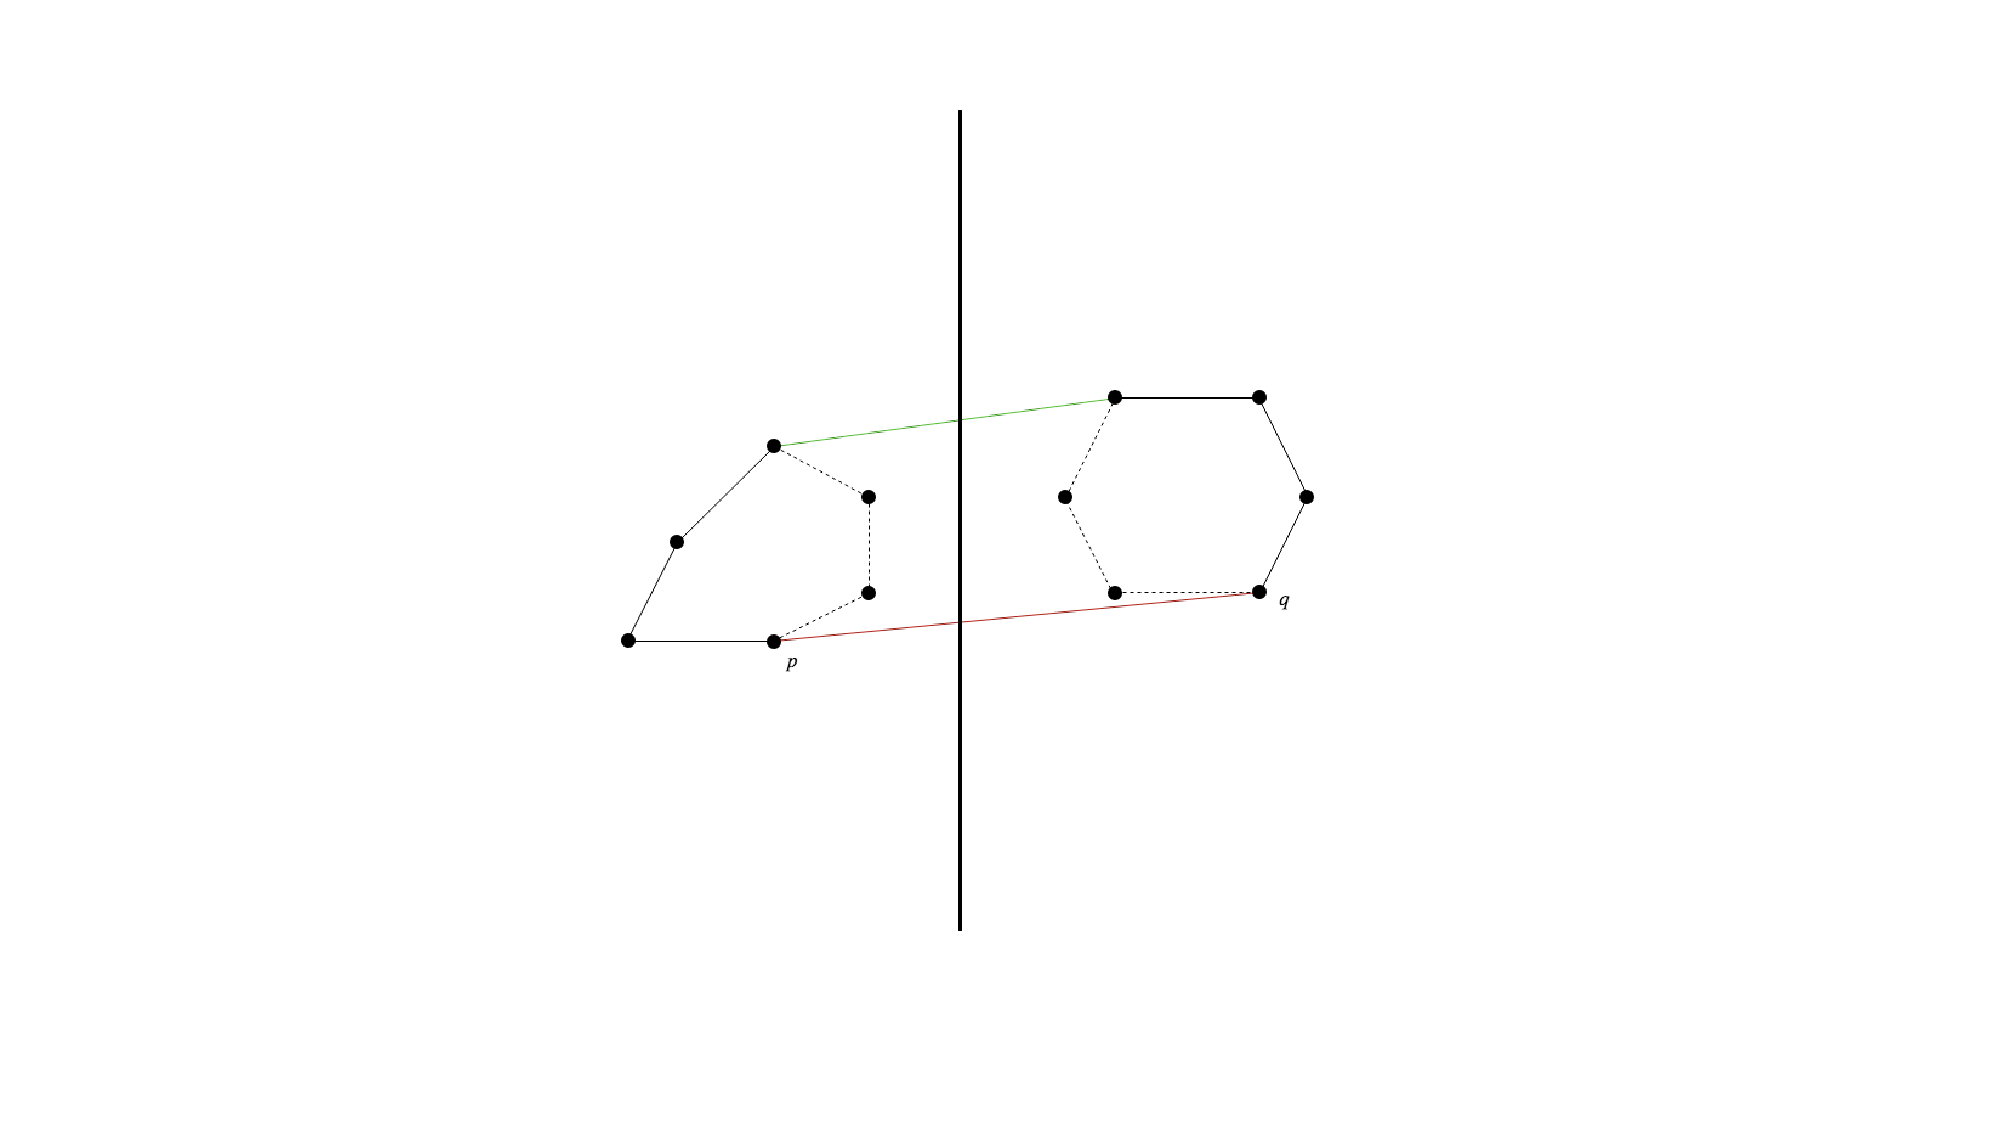
\includepdf[pages=-]{convexpolygon-merging.pdf}
	  	
	
\end{itemize}
 
Now use this to design a D\&C algorithm to find   convex hull of a set on $n$ points. Prove its correctness and establish its time complexity.  



%\includepdf[pages=-]{convexpolygon-compressed.pdf}

%\begin{center}
%\noindent{\bf End of Assignment 1.}
%\end{center}

\end{document}